\documentclass[sigconf, anonymous, review]{acmart}

%% Include any additional packages here
\usepackage{graphicx}
\usepackage{booktabs}
\usepackage{amsmath}
\usepackage{tikz}
\usepackage{pgfplots}
\pgfplotsset{compat=1.18}
\usetikzlibrary{shapes.geometric, arrows.meta, positioning, fit, backgrounds, calc}
\usepackage{multirow}
\usepackage{xcolor}
\emergencystretch=1.5em

\begin{document}

\title{PRONOIA: Event-Driven Financial Reasoning with Market-Verifiable Rewards}

\author{Anonymous Authors}
\affiliation{\institution{Anonymous Institution}}
\email{anonymous@example.com}

\renewcommand{\shortauthors}{Anonymous}

\begin{abstract}
Event-driven equity trading is shifting from speed alpha to cognitive alpha: reading an announcement's implications more deeply than the market. Two gaps persist: classical event studies are post-hoc and discard event structure, while LLM-based analysis is validated almost universally by LLM-as-judge, whose blind spots mirror the evaluatee's.

We present PRONOIA, an event-driven financial reasoning agent deployed as an open-source Web platform, built on three pillars: (i)~an \emph{Event Reasoning Chain} (ERC) architecture formalizing events as state transitions propagated over an economic graph; (ii)~a \emph{Predict--Assert--Verify} (PAV) contract decomposing each prediction into 3--6 falsifiable claims over measurable indicators; and (iii)~\emph{Reinforcement Learning with Verifiable Rewards} (RLVR) settling every claim against post-event market data. On 1,034 time-split out-of-sample A-share events (2024--2026), a rule-driven backtest attains 70.3\% direction accuracy with market confirmation the strongest meta-signal (+18.7pp); PAV-RLVR LoRA improves claim accuracy 57.3\%$\to$63.2\% (+5.9pp, paired bootstrap $p<0.01$) with joint Brier (0.283$\to$0.254) and ECE (0.163$\to$0.107) gains. The model excels at falsifiable claims (significance family 79.1\%, FALSE-side 70.9\%) but lags on momentum claims (TRUE-side 53.0\%); a controlled ablation shows residual-bias rewards induce reward hacking ($-2.29$pt OOS), an empirical caution for financial RL design.

\end{abstract}

\ccsdesc[500]{Computing methodologies~Reinforcement learning}
\ccsdesc[300]{Information systems~Expert systems}
\ccsdesc[300]{Applied computing~Economics}

\keywords{Event-driven financial reasoning, LLM agents, financial world models, RLVR, event study methodology, Web-based AI agents}

\begin{teaserfigure}
\centering
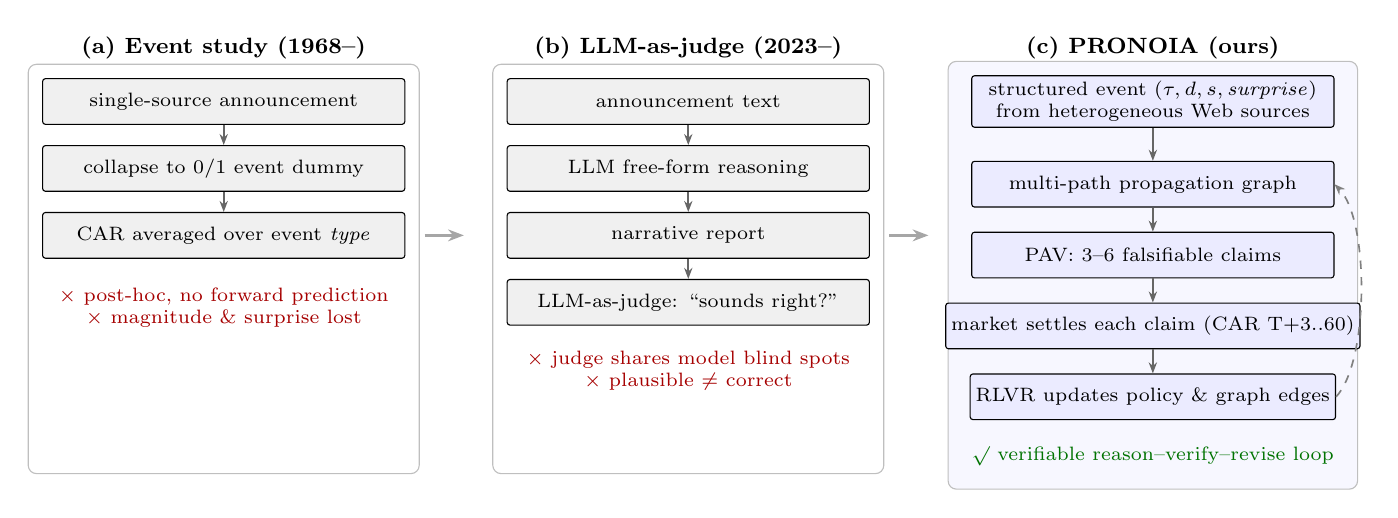
\begin{tikzpicture}[
    eb/.style={draw, rounded corners=1pt, minimum width=4.6cm, minimum height=0.58cm, align=center, font=\scriptsize, inner sep=2pt},
    earr/.style={-{Stealth[length=1.4mm]}, semithick, black!60},
    ttl/.style={font=\footnotesize\bfseries, align=center},
    neg/.style={font=\scriptsize, text=red!65!black, align=center},
    good/.style={font=\scriptsize, text=green!45!black, align=center},
    pnl/.style={draw=black!25, rounded corners=3pt, inner sep=5pt},
    evo/.style={-{Stealth[length=2mm]}, very thick, black!35}
]
    % ===== Panel (a): Event study =====
    \node[eb, fill=black!6] (a1) at (0,0) {single-source announcement};
    \node[eb, fill=black!6] (a2) at (0,-0.85) {collapse to 0/1 event dummy};
    \node[eb, fill=black!6] (a3) at (0,-1.7) {CAR averaged over event \emph{type}};
    \node[neg] (a4) at (0,-2.62) {$\times$~post-hoc, no forward prediction\\$\times$~magnitude \& surprise lost};
    \draw[earr] (a1) -- (a2);
    \draw[earr] (a2) -- (a3);
    \node[ttl] at (0,0.68) {(a)~Event study (1968--)};
    \coordinate (abot) at (0,-4.55);
    % ===== Panel (b): LLM-as-judge =====
    \node[eb, fill=black!6] (b1) at (5.9,0) {announcement text};
    \node[eb, fill=black!6] (b2) at (5.9,-0.85) {LLM free-form reasoning};
    \node[eb, fill=black!6] (b3) at (5.9,-1.7) {narrative report};
    \node[eb, fill=black!6] (b4) at (5.9,-2.55) {LLM-as-judge: ``sounds right?''};
    \node[neg] (b5) at (5.9,-3.42) {$\times$~judge shares model blind spots\\$\times$~plausible $\neq$ correct};
    \draw[earr] (b1) -- (b2);
    \draw[earr] (b2) -- (b3);
    \draw[earr] (b3) -- (b4);
    \node[ttl] at (5.9,0.68) {(b)~LLM-as-judge (2023--)};
    \coordinate (bbot) at (5.9,-4.55);
    % ===== Panel (c): PRONOIA =====
    \node[eb, fill=blue!8] (c1) at (11.8,0) {structured event $(\tau,d,s,\mathit{surprise})$\\from heterogeneous Web sources};
    \node[eb, fill=blue!8] (c2) at (11.8,-1.05) {multi-path propagation graph};
    \node[eb, fill=blue!8] (c3) at (11.8,-1.95) {PAV: 3--6 falsifiable claims};
    \node[eb, fill=blue!8] (c4) at (11.8,-2.85) {market settles each claim (CAR T+3..60)};
    \node[eb, fill=blue!8] (c5) at (11.8,-3.75) {RLVR updates policy \& graph edges};
    \node[good] (c6) at (11.8,-4.5) {$\surd$~verifiable reason--verify--revise loop};
    \draw[earr] (c1) -- (c2);
    \draw[earr] (c2) -- (c3);
    \draw[earr] (c3) -- (c4);
    \draw[earr] (c4) -- (c5);
    \draw[earr, dashed, gray] (c5.east) .. controls (14.55,-3.3) and (14.55,-1.5) .. (c2.east);
    \node[ttl] at (11.8,0.68) {(c)~PRONOIA (ours)};
    \coordinate (cbot) at (11.8,-4.55);
    % ===== Evolution arrows between panels =====
    \draw[evo] (2.55,-1.7) -- (3.05,-1.7);
    \draw[evo] (8.45,-1.7) -- (8.95,-1.7);
    % ===== Panel frames =====
    \begin{scope}[on background layer]
        \node[pnl, fit=(a1)(a4)(abot)] {};
        \node[pnl, fit=(b1)(b5)(bbot)] {};
        \node[pnl, fill=blue!3, fit=(c1)(c6)(cbot)] {};
    \end{scope}
\end{tikzpicture}
\caption{Three paradigms of event-driven financial analysis. (a)~Event studies average CAR by event type---rigorous but post-hoc. (b)~LLM analysis restores event richness but is validated by a judge sharing the evaluatee's blind spots. (c)~PRONOIA structures each event, propagates it over an economic graph, and lets post-event market data settle every claim---closing the reason--verify--revise loop.}
\label{fig:paradigm}
\end{teaserfigure}

\maketitle

\section{Introduction}
\label{sec:intro}

Every trading day, hundreds of corporate disclosures hit the Web---earnings surprises, contract wins, guidance revisions, policy shifts---and each triggers the same race: who reads \emph{what the announcement means} most accurately. Event-driven trading has shifted from \emph{speed alpha}, won by co-location and low-latency feeds, to \emph{cognitive alpha}, won by reasoning more deeply about magnitude, wording, surprise, and cross-sector transmission. But depth does not scale: a skilled analyst can work through only a handful of events per day, and this coverage--depth trade-off is precisely where event-driven performance is capped.

Large language models are the natural technology to break this trade-off---they parse full filings in seconds, detect nuanced tone changes, and sketch transmission chains no template anticipates. Figure~\ref{fig:paradigm} positions the field. The classical event study~(a) is rigorous but post-hoc: it averages over event \emph{types} and cannot say what \emph{this} event will do. LLM-based analysis~(b) restores event richness but is validated almost universally by an LLM judge that shares the evaluatee's blind spots. This paper realizes the missing paradigm~(c): an agent whose every prediction is \emph{settled by the market itself}.

\subsection{Relevance to the Web}

The central scientific challenge in this work is \emph{created} by the Web, not merely hosted on it. Three Web-specific properties make the problem what it is.

\emph{(i) Web-source heterogeneity is the core difficulty.} Financial information never arrives as one authoritative record: the same event is disclosed across exchange announcements, newswires, filings, social media, and macro-data portals that differ in format, latency, granularity, and reliability. Reconstructing a single structured state from these conflicting, continuously updated Web sources---and measuring its departure from what the market already expects---is a Web-scale data-integration and trust problem. It is precisely this heterogeneity that defeats the traditional event-study pipeline, which assumes a clean, single-source event signal.

\emph{(ii) The Web is the ground-truth feedback channel.} The market is a Web-mediated information-aggregation system: prices and abnormal returns are emergent artifacts of continuously published, time-stamped Web data. The Web therefore supplies not only the agent's inputs but also the \emph{verification signal} that settles every prediction. PRONOIA closes this loop---agent reasoning is rewarded against market data as it is published---which makes it an instance of online, real-world reinforcement learning \emph{on the live Web} rather than offline simulation. This is why the strongest meta-signal we measure is market confirmation itself (+18.7pp).

\emph{(iii) Web non-stationarity defeats static evaluation.} Sources, formats, and return distributions shift continuously, so any benchmark frozen at collection time misrepresents deployed agent behaviour. We therefore evaluate reasoning strategies through an online, continuously updated arena over live Web data.

Taken together, these properties place the work squarely in the \emph{Web Infrastructure and Agentic Systems} track: instead of treating the Web as a passive data source, we study how autonomous agents can reason over, and be verified by, the evolving Web.

\subsection{Two Challenges}

Two gaps separate the current state from paradigm~(c).

\textbf{Ch1: events are stripped of structure and studied in isolation.} The five-step event-study pipeline~\cite{fama1969}---define event, estimation window, market model, AR/CAR, significance test---has remained structurally unchanged for over half a century~\cite{ball1968}. It collapses announcements into 0/1 dummies, discarding magnitude, wording, and the market-surprise component that actually moves prices~\cite{kuttner2001}; and it treats events as independent~\cite{kolari2010}, although markets react through multi-layer channels (``rate cut $\to$ developer financing improves $\to$ building-material demand rises'') and systematically underreact to indirect effects~\cite{cohen2008}. The pipeline has no slot for either.

\textbf{Ch2: LLM reasoning has no external ground truth.} LLM analyses address Ch1 but validate with LLM-as-judge: evaluator and evaluatee share error modes, plausible wording games the judge, and ``sounds reasonable'' $\neq$ ``is correct.'' We measure this gap directly in \S\ref{sec:judgevalidity}: given identical information, an independent judge agrees with the evaluatee on 87.7\% of claims yet reaches only $\kappa = 0.199$ against market truth. Without an objective settlement signal, reasoning quality can be neither measured nor improved by training.

These gaps motivate four research questions, answered in \S\ref{sec:experiments}:
\begin{itemize}
    \item \textbf{RQ1 (Signal):} do structured events, combined with market confirmation, carry more verifiable price signal than type-level priors alone?
    \item \textbf{RQ2 (Learning):} can RLVR on market-settled claims improve out-of-sample reasoning over the untrained base?
    \item \textbf{RQ3 (Conditions):} under which event types, claim families, and confidence regimes do the gains concentrate---or reverse?
    \item \textbf{RQ4 (Failure):} what failure modes do reward design and event reasoning expose under controlled comparison?
\end{itemize}

Table~\ref{tab:comparison} situates PRONOIA among event-driven financial AI systems: reported direction accuracy saturates at 55--62\%, consistent with the limited headroom of single-hop ``event $\to$ reaction'' mappings scored by non-verifiable signals.

\begin{table}[t]
\centering\footnotesize
\caption{Comparison with event-driven financial AI systems. ACC = direction accuracy on respective test sets.}
\label{tab:comparison}
\setlength{\tabcolsep}{3pt}
\begin{tabular}{@{}p{1.75cm}p{1.75cm}p{3.15cm}c@{}}
\toprule
System & Approach & Limitation & ACC \\
\midrule
FinHEAR~\cite{finhear2025} & Historical analog & Single-chain, no multi-path & 58--62\% \\
FinKario~\cite{finkario2025} & KG retrieval & Static KG, retrieval-only & 58.1\% \\
Trading\-Agents~\cite{tradingagents2024} & Multi-agent vote & Not event-driven & $\sim$55\% \\
Janus-Q~\cite{janusq2026} & Gated PnL reward & Episode-level, no per-claim check & 58.7\% \\
Argus~\cite{argus2026} & LLM-as-judge & Judge shares errors & --- \\
\midrule
\textbf{PRONOIA} & Graph + PAV + RLVR & US OOS limited & \textbf{63.2\%} \\
\bottomrule
\end{tabular}
\end{table}

\subsection{The PRONOIA Approach}

We present PRONOIA, an event-driven financial reasoning agent built on three pillars (Figure~\ref{fig:paradigm}c):

\begin{enumerate}
    \item \textbf{Structured events.} Each event is a structured information shock $(type, direction, strength, surprise)$ reconstructed from heterogeneous Web sources---not a 0/1 dummy---and serves as input to multi-path propagation.
    \item \textbf{Propagation-graph reasoning.} Economic logic is encoded as a DAG whose nodes are macro variables, sectors, and assets and whose edges are pre-built transmission mechanisms (interest-rate, supply--demand, industry-chain, capital-flow). Multi-path \emph{search and assembly} replaces free-form generation.
    \item \textbf{Market-verifiable claims.} Every prediction is decomposed into falsifiable claims settled by post-event CAR data---never by LLM self-assessment---and the settlements train the agent and recalibrate graph edges, closing the reason $\to$ verify $\to$ revise loop.
\end{enumerate}

\subsection{Contributions}

\begin{enumerate}
    \item \textbf{ERC architecture:} a four-layer Event Reasoning Chain (Perception $\to$ Reasoning $\to$ Decision $\to$ Evolution) operating on the Event--Transmission--Position triple, formalizing the propagation graph as the financial analogue of a world model's transition function.
    \item \textbf{PAV-RLVR framework:} a Predict--Assert--Verify contract decomposing each prediction into 3--6 claims over measurable indicators (CAR, benchmark returns, $p$-values across T+3/7/15/30/60), trained with RLVR against objective market settlements.
    \item \textbf{Controlled validation} on 1,034 time-split out-of-sample A-share events (2024--2026): rule-driven backtest reaches 70.3\% direction accuracy with market confirmation the strongest meta-signal (+18.7pp); PAV-RLVR LoRA improves claim accuracy 57.3\%$\to$63.2\% (+5.9pp, paired bootstrap $p<0.01$) with joint Brier and ECE gains.
    \item \textbf{Reward-hacking documentation:} a controlled ablation in which residual-bias correction rewards \emph{improve} training reward yet \emph{reduce} OOS accuracy by 2.29pt---an empirical caution for financial RL design.
\end{enumerate}

\section{Related Work}

\subsection{Event-Driven Financial Analysis}

The event study of Ball \& Brown~\cite{ball1968} and Fama et al.~\cite{fama1969} remains the empirical cornerstone of event analysis, and its limitations are well documented: event dummies discard the surprise component that moves prices~\cite{kuttner2001}, cross-sectional CAR correlation inflates test statistics~\cite{kolari2010}, and the pipeline offers no slot for economic transmission. Financial NLP supplies richer event representations---detection and coreference (MAVEN~\cite{maven2020}, MAVEN-ERE~\cite{mavenere2022}), document-level extraction (Doc2EDAG~\cite{doc2edag2019}, DCFEE~\cite{dcfee2018}), and event-enhanced knowledge graphs (FinKario~\cite{finkario2025})---but stops at the \emph{perception} layer: structured events are produced without a reasoning layer that propagates them or a verification layer that settles predictions. PRONOIA's contribution is exactly these two missing layers.

Among LLM systems targeting event-driven prediction (Table~\ref{tab:comparison}, \S\ref{sec:intro}), FinHEAR~\cite{finhear2025} retrieves historical analogs along a single chain; FinKario~\cite{finkario2025} retrieves from a static knowledge graph; TradingAgents~\cite{tradingagents2024} aggregates multi-agent votes that are not event-conditioned; Argus~\cite{argus2026} validates with LLM-as-judge. Closest to PRONOIA is the concurrent Janus-Q~\cite{janusq2026}, which likewise trains on event--CAR pairs with a gated trading reward. It differs in three ways: (i)~its prediction target is a trading action validated end-to-end by PnL, whereas PAV decomposes each prediction into 3--6 independently settled claims, exposing \emph{which} component fails; (ii)~it models no explicit multi-path transmission; and (iii)~it reports aggregate trading metrics, whereas we additionally analyze calibration and document a reward-hacking failure mode that aggregate metrics would mask (\S\ref{sec:ablation}).

\subsection{LLM Agents with Verifiable Rewards}

Web agents navigate realistic Web tasks~\cite{webarena2023, workarena2024, visualwebarena2024}, but operate in simulated or static environments whose rewards are programmatic checkers. RAG~\cite{rag2020} grounds generation in retrieved documents, and tool-use benchmarks~\cite{toolbench2023, api2023} score whether API calls succeed. PRONOIA differs on the reward side: the agent reasons over live Web financial data (85+ data skills) and is rewarded by \emph{emergent market outcomes} published on the Web---a continuously updating ground truth that neither a static checker nor a cached snapshot can provide. Retrieval is likewise structured (graph mechanisms rather than document similarity) and generation is verifiable (settled claims rather than grounded text).

RLVR~\cite{rlvr2025} replaces self-evaluation with externally checkable rewards; in finance, AlphaAgent~\cite{alphaagent2025} and FactorMiner~\cite{factorminer2026} apply related ideas to alpha mining. PAV pushes verification from episode level (did the strategy profit?) to claim level (did \emph{each} assertion hold?), which both localizes error and---as \S\ref{sec:ablation} shows---is the guardrail between RLVR and reward hacking. Finally, the propagation graph borrows the world-model view from robotics~\cite{ha2018, schrittwieser2020}: market state plus a structured-event action transitions through the graph and terminates in market verification, with Navigator search as planning.

\section{PRONOIA}

\subsection{System Overview}

PRONOIA is deployed as an open-source Web application (Python 3.10+ backend, React 18 frontend) with the following production components:

\begin{itemize}
    \item \textbf{Conversational Research Workbench:} Researchers interact through a chat interface; cases are persisted in SQLite with full history, enabling refresh-resistant research sessions and follow-up questioning.
    \item \textbf{85+ Real Data Skills:} Market data (akshare, yfinance), news, announcements, financials, macro indicators, and event study methods (AR/CAR computation)---zero mock data.
    \item \textbf{Research Team Mode:} Planner decomposes deep questions $\to$ multiple expert agents execute in parallel $\to$ synthesis $\to$ reviewer cross-checks data facts vs.\ model inference.
    \item \textbf{Artifact System:} Tool results auto-generate charts, data tables, evidence cards, and one-click research reports.
    \item \textbf{Event-Driven Backtesting Platform:} Real events + Oracle T+3$\sim$T+60 CAR labels, Strict/Lenient dual-metric ACC, Wilson CI.
    \item \textbf{Arena Horizontal Evaluation:} Multi-run comparison on same dataset---ranking, radar charts, significance tests, head-to-head analysis, cost-effectiveness Pareto frontier.
    \item \textbf{Security:} LLM keys stored only in backend \texttt{.env}, never transmitted to browser.
\end{itemize}

The platform has been iteratively developed through 13 versions (v3.0--v3.13) over 6 months, with the Arena evaluation system and multi-horizon CAR labeling added in recent versions based on experimental feedback. The Arena subsystem deserves emphasis: it addresses a critical gap in LLM evaluation---most systems report single-run results without statistical validation. Arena combines 18+ pluggable metrics in three tiers with Wilson confidence intervals, paired bootstrap tests, and FDR correction for multiple comparisons, making it trivial to verify whether an improvement is significant or noise.

\subsection{Data Pipeline}

\begin{figure}[t]
\centering
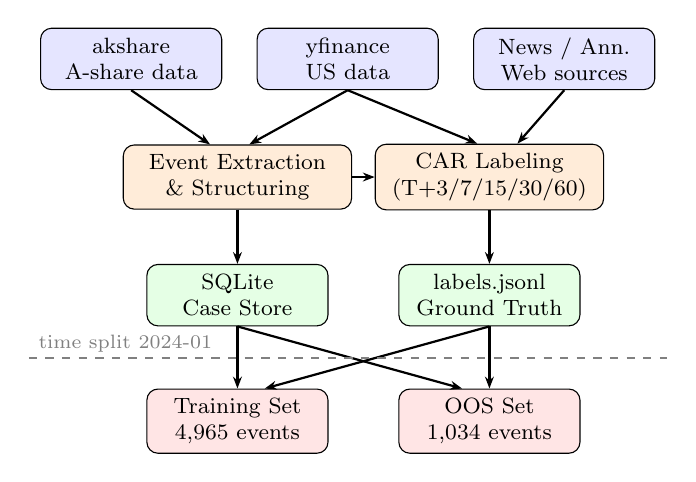
\begin{tikzpicture}[
    box/.style={draw, rounded corners, minimum width=2.3cm, minimum height=0.78cm, align=center, font=\footnotesize},
    arrow/.style={-{Stealth[length=1.5mm]}, thick}
]
    % Row 1: input sources
    \node[box, fill=blue!10] (ak) at (0,0) {akshare\\A-share data};
    \node[box, fill=blue!10] (yf) at (2.75,0) {yfinance\\US data};
    \node[box, fill=blue!10] (news) at (5.5,0) {News / Ann.\\Web sources};

    % Row 2: processing
    \node[box, fill=orange!15, minimum width=2.9cm] (extract) at (1.35,-1.5) {Event Extraction\\\& Structuring};
    \node[box, fill=orange!15, minimum width=2.9cm] (label) at (4.55,-1.5) {CAR Labeling\\(T+3/7/15/30/60)};

    % Row 3: storage
    \node[box, fill=green!10] (sqlite) at (1.35,-3.0) {SQLite\\Case Store};
    \node[box, fill=green!10] (jsonl) at (4.55,-3.0) {labels.jsonl\\Ground Truth};

    % Row 4: output
    \node[box, fill=red!10] (train) at (1.35,-4.6) {Training Set\\4,965 events};
    \node[box, fill=red!10] (oos) at (4.55,-4.6) {OOS Set\\1,034 events};

    % Arrows
    \draw[arrow] (ak.south) -- (extract.130);
    \draw[arrow] (yf.south) -- (extract.70);
    \draw[arrow] (yf.south) -- (label.110);
    \draw[arrow] (news.south) -- (label.50);
    \draw[arrow] (extract) -- (label);
    \draw[arrow] (extract) -- (sqlite);
    \draw[arrow] (label) -- (jsonl);
    \draw[arrow] (sqlite.south) -- (train.north);
    \draw[arrow] (jsonl.south) -- (oos.north);
    \draw[arrow] (sqlite.south) -- (oos.130);
    \draw[arrow] (jsonl.south) -- (train.50);

    % Time split
    \draw[dashed, thick, gray] (-1.3,-3.8) -- (6.8,-3.8);
    \node[font=\scriptsize, text=gray, anchor=west] at (-1.3,-3.62) {time split 2024-01};
\end{tikzpicture}
\caption{PRONOIA data pipeline: Web data sources $\to$ event extraction and CAR labeling $\to$ time-split storage for training and evaluation.}
\label{fig:pipeline}
\end{figure}

Figure~\ref{fig:pipeline} shows the data pipeline. Events are extracted from Web sources, structured into the ETP format, and labeled with multi-horizon CAR ground truth. The time-split ensures no lookahead bias: training uses events before 2024-01, OOS evaluation uses events after.

\subsection{Event Reasoning Chain}

\begin{figure}[t]
\centering
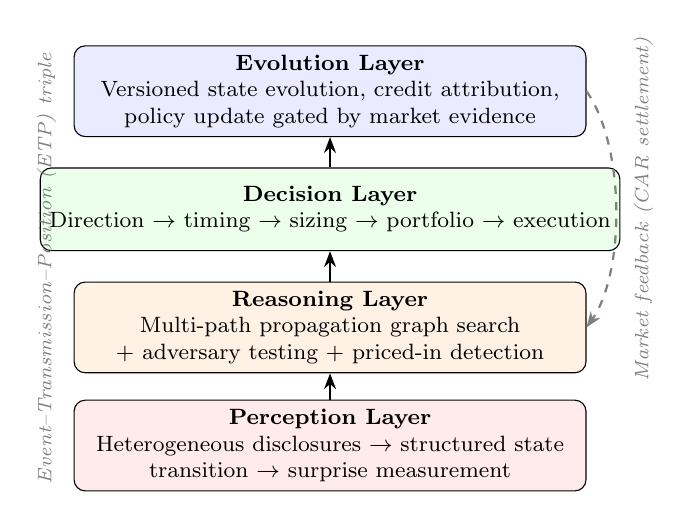
\begin{tikzpicture}[
    layer/.style={draw, rounded corners, minimum width=6.5cm, minimum height=1.05cm, align=center, font=\footnotesize},
    arrow/.style={-{Stealth[length=2mm]}, thick},
    sidelabel/.style={font=\scriptsize\itshape, text=gray}
]
    % Layers
    \node[layer, fill=blue!8] (l4) at (0,0) {\textbf{Evolution Layer}\\Versioned state evolution, credit attribution,\\policy update gated by market evidence};
    \node[layer, fill=green!8] (l3) at (0,-1.5) {\textbf{Decision Layer}\\Direction $\to$ timing $\to$ sizing $\to$ portfolio $\to$ execution};
    \node[layer, fill=orange!10] (l2) at (0,-3.0) {\textbf{Reasoning Layer}\\Multi-path propagation graph search\\+ adversary testing + priced-in detection};
    \node[layer, fill=red!8] (l1) at (0,-4.5) {\textbf{Perception Layer}\\Heterogeneous disclosures $\to$ structured state\\transition $\to$ surprise measurement};

    % Arrows
    \draw[arrow] (l1) -- (l2);
    \draw[arrow] (l2) -- (l3);
    \draw[arrow] (l3) -- (l4);

    % Side labels
    \node[sidelabel, rotate=90] at (-3.6,-2.25) {Event--Transmission--Position (ETP) triple};

    % Feedback loop
    \draw[arrow, dashed, gray] (l4.east) .. controls (3.75,-0.7) and (3.75,-2.3) .. (l2.east);
    \node[sidelabel, rotate=90] at (3.98,-1.5) {Market feedback (CAR settlement)};
\end{tikzpicture}
\caption{PRONOIA's four-layer Event Reasoning Chain (ERC) architecture. The system operates on the Event--Transmission--Position (ETP) triple as atomic logic unit, with market feedback closing the evolution loop.}
\label{fig:erc}
\end{figure}

PRONOIA's four-layer architecture (Figure~\ref{fig:erc}) operates on the Event--Transmission--Position (ETP) triple:

\begin{enumerate}
    \item \textbf{Perception:} Heterogeneous disclosures $\to$ structured state transition $\to$ surprise measurement.
    \item \textbf{Reasoning:} Multi-path Propagation Graph search + adversary testing + priced-in detection.
    \item \textbf{Decision:} Direction $\to$ timing $\to$ sizing $\to$ portfolio $\to$ execution.
    \item \textbf{Evolution:} Versioned state evolution, credit attribution, policy update gated by market evidence.
\end{enumerate}

This paper focuses on Layers 2 (Reasoning) and 4 (Evolution via RLVR), with Layers 1 and 3 providing input context.

\begin{definition}[Event]
An event $e$ is a state transition $X_e^- \to X_e^+$ of a declared system $S$ at time $t_e$, with ex-ante benchmark $B_e$. The \emph{surprise} is $X_e^+ - B_e$, not $X_e^+ - X_e^-$.
\end{definition}

This resolves the common confusion: a large state change (guidance revision \$10--11B $\to$ \$8--9B) is not a large surprise if the market expected \$8.5B.

\begin{definition}[Event Boundary]
Boundary = System$(S)$ + State Representation$(X)$ + Analytical Scale$(\sigma)$. A single earnings release can be one event at filing scale or several at item scale (revenue, EPS, guidance changes).
\end{definition}

\subsection{Propagation Graph}

$G = (V, A)$ is a DAG where:
\begin{itemize}
    \item \textbf{Nodes $V$:} Each $v$ contains (subject, expected direction and magnitude, time window), from macro variables to sectors to individual assets.
    \item \textbf{Edges $A$:} Each $a = (u,v,label)$, $label \in \{+1, -1\}$, carrying a conditional transmission probability
    \[ P(B_{up}|A_{up}) = N(A_{up} \wedge B_{up})\,/\,N(A_{up}), \]
    fused via Bayesian update $P_{\mathrm{new}} = 0.7\,P_{\mathrm{prior}} + 0.3\,P_{\mathrm{observed}}$.
\end{itemize}

Three edge-source tiers: (a)~prior historical statistics, (b)~online recent CAR observations, (c)~Navigator real-time reasoning.

\begin{figure}[t]
\centering
\resizebox{\columnwidth}{!}{%
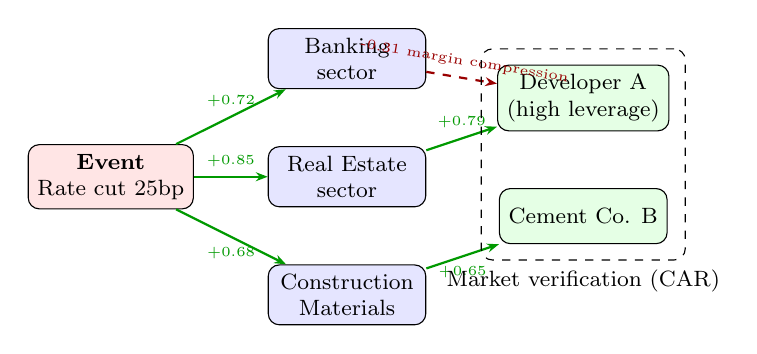
\begin{tikzpicture}[
    node/.style={draw, rounded corners, minimum width=2cm, minimum height=0.7cm, align=center, font=\footnotesize},
    edge/.style={-{Stealth[length=1.5mm]}, thick},
    posedge/.style={edge, green!60!black},
    negedge/.style={edge, red!60!black, dashed}
]
    % Nodes
    \node[node, fill=red!10] (event) at (0,0) {\textbf{Event}\\Rate cut 25bp};
    \node[node, fill=blue!10] (bank) at (3,1.5) {Banking\\sector};
    \node[node, fill=blue!10] (realestate) at (3,0) {Real Estate\\sector};
    \node[node, fill=blue!10] (materials) at (3,-1.5) {Construction\\Materials};
    \node[node, fill=green!10] (stock1) at (6,1.0) {Developer A\\(high leverage)};
    \node[node, fill=green!10] (stock2) at (6,-0.5) {Cement Co. B};
    
    % Edges
    \draw[posedge] (event) -- node[above, font=\tiny]{+0.72} (bank);
    \draw[posedge] (event) -- node[above, font=\tiny]{+0.85} (realestate);
    \draw[posedge] (event) -- node[below, font=\tiny]{+0.68} (materials);
    \draw[posedge] (realestate) -- node[above, font=\tiny]{+0.79} (stock1);
    \draw[posedge] (materials) -- node[below, font=\tiny]{+0.65} (stock2);
    \draw[negedge] (bank) -- node[above, font=\tiny, sloped]{-0.31 margin compression} (stock1);
    
    % Verification
    \node[draw, dashed, rounded corners, fit=(stock1) (stock2), inner sep=0.2cm, label={[font=\footnotesize]below:Market verification (CAR)}] (verify) {};
\end{tikzpicture}}
\caption{Example Propagation Graph for a rate cut event. Nodes represent sectors/assets with expected direction and magnitude; edges represent transmission mechanisms with conditional probabilities. Dashed red edge shows a competing negative path (margin compression). The final positions are verified against actual post-event CAR data.}
\label{fig:propagation}
\end{figure}

Figure~\ref{fig:propagation} illustrates a concrete propagation graph. The rate cut event transmits through multiple paths: direct banking sector impact, real estate financing improvement, and construction materials demand. Each edge weight is continuously calibrated by market feedback.

\subsection{Navigator-Searcher Protocol}

Six-step collaboration over $G$:
\begin{enumerate}
    \item Navigator decomposes event $e$ into sub-problems, dispatching one Searcher per sub-problem.
    \item Each Searcher, adopting a market-participant persona (long/short/arbitrageur/regulator/retail), traces one propagation chain.
    \item Outputs merged into DAG: deduplicated, cross-referenced, marked with verification status.
    \item Navigator identifies unconnected components; prompts additional Searchers.
    \item Market verification via CAR + dose-response + volume/volatility validates or falsifies each path.
    \item Verified paths form final reasoning graph; emit directional, magnitude, and confidence judgments.
\end{enumerate}

Key choices: DAG not tree (multiple causes per effect); market posterior not LLM voting as ground truth; game-theoretic branching with heterogeneous personas.

\subsection{PAV Output Contract}

\textbf{Predict:} Input: event structured fields + as\_of research context (strictly no post-event data: T0 return, pre-5/pre-20 drift, CAR to T0) + measurable indicator panel (30 indicators defined, values withheld).

\textbf{Assert:} Model proposes 3--6 verifiable claims: (indicator, horizon, threshold, TRUE/FALSE, confidence, reasoning\_chain). Five families across T+3/7/15/30/60: \texttt{car\_t\{h\}}, \texttt{ret\_t\{h\}}, \texttt{bm\_ret\_t\{h\}}, \texttt{car\_t\{h\}\_pvalue}, \texttt{car\_avg\_*}.

\textbf{Verify:} Each claim objectively settled against labels.jsonl. Compute claim-level accuracy, Brier, ECE, verifiability, diversity.

The departure: PAV shifts core metric from ``did you guess direction right?'' to ``are your claims testable and correct?'' Evaluation goes from event-level to claim-level.

\subsection{RLVR Training}
\label{sec:rlvr-training}

Qwen3-8B (bf16, backbone frozen, LoRA rank 16) trained with GRPO~\cite{grpo2025} via RLVR~\cite{rlvr2025}. Per event: $G=4$ candidates, parsed into claims, settled against labels.

Reward is six-element tuple (R0--R5): claim accuracy (core), confidence calibration (Brier), verifiability ratio, diversity (family coverage), format compliance, length penalty.

\textbf{Reward variants:} \textbf{PAVR-C} adds five residual bias corrections (B3: hard-negative targeting; B4/B5: distribution residual correction; B7: claim combination quality; T3: format bonus); \textbf{PAVR} uses settlement-only reward without these corrections.

\textbf{Training:} GRPO (TRL 0.17) + Unsloth acceleration (in-process vLLM, weight sharing, Standby mode, $\sim$2.3$\times$ speedup). Batch 8/device $\times$ grad-accum 2 = 16 completions/step (4 events $\times$ 4 candidates). LR 1e-5, cosine annealing. 1 epoch = 1,241 steps $\approx$ 4,965 events. Seed 42. Single RTX 4090 (48GB), 10--12h/condition.

\section{Experiments}
\label{sec:experiments}

This section answers RQ1--RQ4 in sequence. \textbf{RQ1} is tested by a rule-driven backtest isolating the marginal value of structured events and market confirmation over type-level priors (\S\ref{sec:backtest}, Table~\ref{tab:backtest}). \textbf{RQ2} is tested by the PAV-RLVR controlled ablation on 1,034 time-split out-of-sample events (\S\ref{sec:ablation}, Table~\ref{tab:main}). \textbf{RQ3} localizes the gains by condition slices---hard negatives, event types, indicator families, and calibration (\S\ref{sec:analysis}). \textbf{RQ4} documents reward hacking and reasoning failures, with claim-level case detail in Appendix~\ref{app:cases}. Each experiment uses the same time-split protocol and settlement machinery described next.

\subsection{Dataset and Protocol}

\begin{table}[t]
\centering\footnotesize
\caption{Dataset statistics (time-split).}
\label{tab:dataset}
\setlength{\tabcolsep}{4pt}
\begin{tabular}{@{}lccp{2.9cm}@{}}
\toprule
Split & Events & Markets & Sources \\
\midrule
Train & 4,965 & CN 4,352 / US 613 & Pre-announcements, M\&A, guidance, macro \\
OOS & 1,034 & CN 1,027 / US 7 & Same, post-2024-01, evaluated once \\
\bottomrule
\end{tabular}
\end{table}

Known biases: US near-absent in OOS; no macro events in OOS; scope limited to CN A-shares.

\textbf{Integrity protocol:} (1)~Strict as\_of: features use only pre-event data, audited; (2)~Time split only, OOS once; (3)~Event-level paired bootstrap (2,000 resamples, weighted); (4)~Claim accuracy weighted by n\_settleable; (5)~Calibration: Brier + 10-bin ECE + confidence-bin actual accuracy.

\subsubsection{Settlement Validity: LLM-as-Judge vs. Market}
\label{sec:judgevalidity}

PAV's premise (Ch2) is that market settlement cannot be replaced by LLM-as-judge. We test this premise directly: an independent judge model, given exactly the same pre-event information as the evaluatee (zero leakage), rules on a sample of already-settled claims; its verdicts are scored against market ground truth.

\begin{table}[t]
\centering\small
\caption{Judge-vs-market validity. An independent judge (GLM-5.3), given the same pre-event information as the evaluatee (zero leakage), rules on 500 sampled settled claims (432 parse into valid verdicts); verdicts are scored against market ground truth.}
\label{tab:judge}
\begin{tabular}{@{}lc@{}}
\toprule
Metric & Value \\
\midrule
Judge accuracy (vs.\ market truth) & 0.625 \\
Cohen's $\kappa$ (judge vs.\ truth) & 0.199 \\
Agreement (judge vs.\ evaluatee) & 0.877 \\
Evaluatee accuracy (same claims) & 0.613 \\
Settled claims judged & 432 / 500 \\
\bottomrule
\end{tabular}
\end{table}

Table~\ref{tab:judge} confirms the premise quantitatively: the judge agrees with the evaluatee on 87.7\% of claims, yet its agreement with market truth is weak ($\kappa = 0.199$) and its accuracy (62.5\%) barely exceeds the evaluatee's own (61.3\% on the same claims). Given identical information, the judge tracks the evaluatee far more closely than it tracks the market---its verdicts measure \emph{plausibility}, not correctness. Only settlement by the market itself supplies the objective signal that RLVR requires.

\subsection{RQ1: Signal Validation via Rule-Driven Backtest}
\label{sec:backtest}

\textbf{Design:} 27 A-share blue chips + 8 sector ETFs, CSI300 benchmark, 2023-01 to 2026-07, 33 events, 20 types, CAR via market model (120d estimation, 20d gap, T+3 holding). We do not claim tradability: transaction costs, slippage, and capacity are deliberately excluded---the backtest serves solely as an \emph{economic-materiality lens} verifying that claim-level directional judgments carry exploitable signal, not as a deployable trading system.

\begin{table}[t]
\centering\footnotesize
\caption{Rule-driven backtest results. S1--S5 implement prior $\to$ market confirmation $\to$ noise removal $\to$ strong-signal focus.}
\label{tab:backtest}
\setlength{\tabcolsep}{4pt}
\begin{tabular}{@{}lccccc@{}}
\toprule
Strategy & N & ACC & 95\% CI & Sharpe & avgCAR \\
\midrule
S1 All & 444 & 51.6\% & [47, 56] & $-$1.01 & $-$0.26\% \\
S2 SectorConfirm & 212 & \textbf{70.3\%} & [64, 76] & 3.21 & +0.71\% \\
S3 StrongEvent & 159 & 71.1\% & [64, 78] & 1.48 & +0.32\% \\
S4 NonPriceIn & 130 & 74.6\% & [67, 82] & 3.85 & +0.65\% \\
S5 StrongNonPriceIn & 85 & \textbf{78.8\%} & [69, 87] & 0.81 & +0.13\% \\
\bottomrule
\end{tabular}
\end{table}

Key findings: (1)~S1 51.6\% $\approx$ random---priors alone cannot trade; (2)~Sector ETF confirmation is the strongest meta-signal (+18.7pp, Sharpe $-$1.01$\to$3.21)---``use market posterior to filter priors''; (3)~Event strength quantifies surprise (routine cuts 47.9\% $<$ random; 924-package cuts 82.6\%); (4)~``Graph can only be used once''---low-ACC events (consumer boost 33.3\%, spike-crash 31.6\%, rate cuts 47.9\%) prove lookup tables fail, motivating online reasoning. In/out-of-sample gap 1.2pp; LOEO 68.0--71.4\%.

\subsection{RQ2: PAV-RLVR Main Results and Reward Ablation}
\label{sec:ablation}

\begin{table}[t]
\centering\small
\caption{PAV-RLVR main results (1,034 OOS events, $t=0.6$). $\uparrow$/$\downarrow$: higher/lower is better; bold marks the better value per row.}
\label{tab:main}
\begin{tabular}{@{}lcc@{}}
\toprule
Metric & Base & PAVR \\
\midrule
\textbf{Claim ACC} $\uparrow$ & 0.5729 & \textbf{0.6322} \\
Brier $\downarrow$ & 0.2826 & \textbf{0.2539} \\
ECE $\downarrow$ & 0.1632 & \textbf{0.1070} \\
Format compliance $\uparrow$ & 0.775 & \textbf{0.842} \\
Settled claims $\uparrow$ & 2,978 & \textbf{3,154} \\
\bottomrule
\end{tabular}
\end{table}

Paired bootstrap: $\Delta$(PAVR $-$ base) = +5.93pt (95\% CI [+3.79, +8.07])---CI excludes zero.

\begin{table}[t]
\centering\small
\caption{Zero-shot API baselines on the same 1,034 OOS events, identical PAV prompt and settlement machinery (temperature 0.6). $\uparrow$/$\downarrow$: higher/lower is better; bold marks the best value per column. GLM and DeepSeek-V4-Pro rows from completed runs; DeepSeek-V4-Flash and Kimi-K3 rows pending.}
\label{tab:external}
\setlength{\tabcolsep}{5pt}
\begin{tabular}{@{}lccccc@{}}
\toprule
Model & Params & ACC $\uparrow$ & Brier $\downarrow$ & ECE $\downarrow$ & Format $\uparrow$ \\
\midrule
Base (Qwen3-8B) & 8B & 0.573 & 0.283 & 0.163 & 0.775 \\
PAVR (ours) & 8B+LoRA & 0.632 & 0.254 & 0.107 & 0.842 \\
\midrule
GLM-5.3 & -- & \textbf{0.643} & \textbf{0.228} & 0.033 & 0.972 \\
GLM-5.3-Flash & -- & 0.621 & 0.232 & \textbf{0.015} & \textbf{0.991} \\
DeepSeek-V4-Pro & -- & 0.593 & 0.239 & 0.018 & 0.995 \\
DeepSeek-V4-Flash & -- & -- & -- & -- & -- \\
Kimi-K3 & -- & -- & -- & -- & -- \\
\bottomrule
\end{tabular}
\end{table}

Table~\ref{tab:external} adds zero-shot API baselines: five frontier models run the identical PAV contract on the same OOS events and are settled by the same machinery. This separates the contribution of market-settlement training from raw model scale. The strongest API baseline, GLM-5.3, edges PAVR on raw claim accuracy (0.643 vs.\ 0.632) and is better calibrated still, so RLVR on verifiable rewards lets an 8B open model close the capacity gap against a $\sim$60$\times$-larger frontier backbone rather than surpass it.

\textbf{US extension panel.} We additionally assemble 44 independently labelled US events (H1~2026: inflation 6, FOMC 4, earnings 12, guidance 12, M\&A 10) and settle the same PAV contract against US data; Table~\ref{tab:usext} reports claim-level accuracy with Wilson 95\% intervals. The API models cluster in a 0.60--0.66 band, mirroring the main panel's far-from-saturation picture. Our own Base and PAVR checkpoints, generated on the same 44 events, sit at the top of the panel: PAVR reaches 0.680 claim accuracy (best on the panel) with Brier 0.220 (also best), a +1.3pp gain over Base (0.667) with substantially better calibration (ECE 0.073 vs.\ 0.139), showing the RLVR benefit transfers to the out-of-market US setting.

\begin{table}[t]
\centering\footnotesize
\caption{US extension panel (44 out-of-market H1-2026 events), same PAV prompt and settlement machinery; claim-level ACC with Wilson 95\% intervals ($n$ = settled claims). Bold: best per column.}
\label{tab:usext}
\setlength{\tabcolsep}{4pt}
\begin{tabular}{@{}lccccc@{}}
\toprule
Model & Claims & ACC $\uparrow$ & 95\% CI & Brier $\downarrow$ & ECE $\downarrow$ \\
\midrule
Base (Qwen3-8B) & 123 & 0.667 & [0.579, 0.744] & 0.236 & 0.139 \\
PAVR (ours) & 125 & \textbf{0.680} & [0.594, 0.755] & \textbf{0.220} & 0.073 \\
\midrule
GLM-5.3 & 220 & 0.659 & [0.594, 0.719] & 0.228 & 0.075 \\
GLM-5.3-Flash & 231 & 0.623 & [0.559, 0.683] & 0.233 & \textbf{0.035} \\
DeepSeek-V4-Pro & 201 & 0.602 & [0.533, 0.667] & 0.239 & 0.063 \\
DeepSeek-V4-Flash & 187 & 0.610 & [0.538, 0.677] & 0.230 & 0.041 \\
Kimi-K3 & 229 & 0.638 & [0.574, 0.697] & 0.232 & 0.060 \\
\bottomrule
\end{tabular}
\end{table}

\begin{table}[t]
\centering\small
\caption{PAVR robustness across random seeds (identical pipeline and OOS set). $\uparrow$/$\downarrow$: higher/lower is better.}
\label{tab:seeds}
\begin{tabular}{@{}lccc@{}}
\toprule
Seed & 42 & 43 & 44 \\
\midrule
Claim ACC $\uparrow$ & 0.6322 & 0.6437 & 0.6318 \\
Brier $\downarrow$ & 0.2539 & 0.2493 & 0.2567 \\
ECE $\downarrow$ & 0.1070 & 0.1008 & 0.1172 \\
\bottomrule
\end{tabular}
\end{table}

Seed robustness is summarized in Table~\ref{tab:seeds}. All three seeds agree within 1.2pt of claim accuracy and below 0.008 Brier, addressing the single-seed risk flagged in \S\ref{sec:audit}.

\textbf{Ablation (reward corrections):} Adding the five residual bias corrections of \S\ref{sec:rlvr-training} to the reward (variant PAVR-C) yields 0.609 claim ACC---\emph{below} PAVR by 2.29pt (95\% CI [+0.78, +3.79]). PAVR-C's gains are confined to format compliance and settled-claim volume; calibration is equivalent. Table~\ref{tab:ablation} consolidates the full comparison.

\subsection{RQ3: Where Do the Gains Concentrate?}
\label{sec:analysis}

\subsubsection{Hard-Negative Subset}

146 events (M\&A success, turnaround, beat, additional issuance, buyback): base 0.5103, PAVR-C 0.5515, \textbf{PAVR 0.5862}. Corrections help +3.5pt on this subset but net negative overall---the ``residual bias correctable by prior'' premise is unsupported.

\begin{figure}[t]
\centering
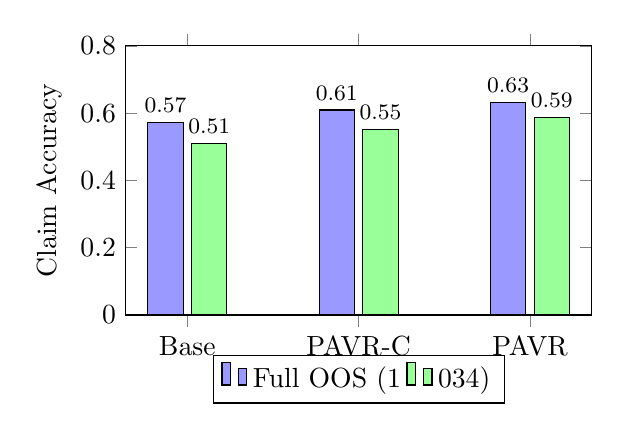
\begin{tikzpicture}
\begin{axis}[
    ybar=3pt,
    bar width=0.45cm,
    width=7.5cm,
    height=5cm,
    ymin=0, ymax=0.8,
    enlarge x limits=0.18,
    ylabel={Claim Accuracy},
    symbolic x coords={Base, PAVR-C, PAVR},
    xtick=data,
    nodes near coords,
    nodes near coords align={vertical},
    every node near coord/.append style={font=\footnotesize},
    legend style={at={(0.5,-0.15)}, anchor=north, legend columns=-1}
]
\addplot[fill=blue!40] coordinates {(Base,0.5729) (PAVR-C,0.6093) (PAVR,0.6322)};
\addplot[fill=green!40] coordinates {(Base,0.5103) (PAVR-C,0.5515) (PAVR,0.5862)};
\legend{Full OOS (1,034), Hard Negatives (146)}
\end{axis}
\end{tikzpicture}
\caption{Claim accuracy comparison: full OOS set vs. hard-negative subset. PAVR achieves best performance on both, with larger margin on hard negatives (+7.6pt vs. base).}
\label{fig:results}
\end{figure}

\subsubsection{By Event Type}

\begin{table}[t]
\centering\small
\caption{Accuracy by event type (CN market).}
\label{tab:bytype}
\begin{tabular}{@{}lcccc@{}}
\toprule
Event Type & Events & Base & PAVR & $\Delta$ \\
\midrule
Earnings beat/miss & 478 & 0.524 & 0.598 & \textbf{+7.4pt} \\
M\&A/spinoff/financing & 373 & 0.618 & 0.661 & +4.4pt \\
Guidance up/down & 169 & 0.632 & 0.679 & +4.8pt \\
Policy rate & 7 & 0.598 & 0.591 & (few) \\
\bottomrule
\end{tabular}
\end{table}

Earnings: largest relative lift (+7.4pt) but lowest absolute (0.598)---strongest priors, hardest cases. M\&A/guidance: highest absolute (0.661, 0.679).

\subsubsection{By Indicator Family $\times$ Horizon}

\begin{table}[t]
\centering\small
\caption{Accuracy by indicator family and horizon.}
\label{tab:byfamily}
\begin{tabular}{@{}lcccc@{}}
\toprule
Slice & Claims & Base & PAVR & $\Delta$ \\
\midrule
Significance ($p$-val) & 944 & 0.614 & \textbf{0.791} & \textbf{+17.7pt} \\
CAR & 1,207 & 0.566 & 0.592 & +2.6pt \\
Benchmark & 647 & 0.411 & 0.498 & +8.7pt \\
Horizon t30 & 675 & 0.622 & \textbf{0.753} & \textbf{+13.1pt} \\
Horizon t7 & 1,154 & 0.559 & 0.619 & +6.0pt \\
Horizon t15 (worst) & 610 & 0.452 & 0.505 & +5.3pt \\
\bottomrule
\end{tabular}
\end{table}

Significance family strongest (+17.7pt to 79.1\%): most A-share CARs insignificant---falsifying significance is the model's strongest move. Weakest: \texttt{bm\_ret\_t15} (0.498, coin-flip). Long-horizon t30 (+13.1pt) vs t15 (+5.3pt): falsifiable long-horizon claims outperform.

\subsubsection{Conditional Analysis}
\label{sec:conditional}

\textbf{Claim count:} 2--3 best (0.690/0.656); 4 drops to 0.569. Constraint should narrow to 3--4.
\textbf{Direction:} FALSE-side \textbf{0.709} (n=1,812) vs TRUE-side \textbf{0.530} (n=1,342). Training reduces TRUE ratio 0.525$\to$0.425---beneficial RL product matching task asymmetry.
\textbf{Extremes:} 293 all-correct (28.3\%, M\&A/earnings); 55 all-wrong (5.3\%, beat/turnaround).
\textbf{Calibration:} Non-monotonic---0.75--0.85 bin actual accuracy only 0.53--0.59 (main ECE contributor); 0.80/0.90 ends reliable (0.777/0.926). Platt post-hoc: ECE 0.085$\to$0.036.

\textbf{Profile:} Excels at FALSE, long-horizon t30, significance, M\&A/guidance, 2--3 claims, confidence 0.80/0.90. Struggles with TRUE momentum, benchmark direction, hard-negatives, 4+ claims, 0.75--0.85 confidence.

\subsection{RQ4: Reward Hacking and Failure Modes}
\label{sec:cases}

RQ4 asks what failure modes reward design and event reasoning expose. Two are documented.

\textbf{Reward hacking.} Corrections' format benefit (+15.5pt, Table~\ref{tab:ablation}) is recoverable by inference-time re-sampling. Training reward \emph{inversely correlates} with OOS accuracy---the model optimizes proxy signals over claim quality. KL, length, and truncation diagnostics are healthy and comparable, ruling out instability. \textbf{Implication: training reward trend cannot validate reward components; OOS adjudication is the only mechanism.}

\begin{table}[t]
\centering\small
\caption{Reward-correction ablation (seed 42, identical pipeline and OOS set). $\uparrow$/$\downarrow$: higher/lower is better; bold marks the better value per arrowed row (ECE equivalent). Training reward is a proxy diagnostic, hence no arrow. $\Delta$: PAVR-C minus PAVR. The corrections win every training- and format-side metric yet lose the only out-of-sample-adjudicated one.}
\label{tab:ablation}
\setlength{\tabcolsep}{5pt}
\begin{tabular}{@{}lccc@{}}
\toprule
 & PAVR & PAVR-C & $\Delta$ \\
\midrule
OOS claim ACC $\uparrow$ & \textbf{0.632} & 0.609 & $-$2.29pt \\
Training reward (last 200 steps, proxy) & 0.69 & 0.90 & +0.21 \\
Format compliance $\uparrow$ & 0.842 & \textbf{0.997} & +15.5pt \\
Settled claims $\uparrow$ & 3,154 & \textbf{4,056} & +902 \\
ECE $\downarrow$ & 0.1070 & 0.1064 & $-$0.0006 \\
\bottomrule
\end{tabular}
\end{table}

Table~\ref{tab:ablation} consolidates the ablation: the corrected reward wins every training-side and format-side metric---higher training reward, near-perfect format compliance, more settled claims---yet loses the only metric adjudicated out of sample. The ACC gap is significant (95\% CI [+0.78, +3.79], paired event-level bootstrap; event-level win/tie/loss 394/302/335 in PAVR's favor). The variant with the higher training reward delivers the lower OOS accuracy.

\textbf{Reasoning failures.} Claim-level tracing of OOS events (three representative cases in Appendix~\ref{app:cases}; full synthesis there) reveals two recurring patterns: (i)~failures concentrate in ``bullish text + T0 positive reaction'' configurations, where the model's prior is momentum but A-share reality is mean reversion---risk paragraphs are \emph{cognitively correct but behaviorally inert}, never converting into hedging claims; and (ii)~upstream context with strong priors contaminates downstream reasoning (individual-stock weakness extrapolated to benchmark direction, near coin-flip), while cross-indicator claims are silently dropped. The success case shows the complementary mechanism: context absorption, claim diversity, and willingness to bet FALSE.

\section{Discussion}
\label{sec:audit}

The two experiments validate one proposition at three levels. First, priors cannot trade: the rule backtest's unconfirmed step S1 (51.6\%) and the untuned base model (0.573) agree that type-level priors carry no exploitable signal. Second, market confirmation purifies: the +18.7pp jump when sector confirmation enters the rule pipeline and the +5.9pt jump when market settlement enters training are the same mechanism---a verifiable filter that removes the reasoning steps the environment can refute---applied at two different sites. Third, the environment demands online reasoning: ``graph once'' cannot anticipate indirect effects, which is why we learn propagation rather than hard-code it, and reward hacking shows that even the reward function itself requires OOS adjudication.

\textbf{Limitations.} The main OOS split contains only seven US events, so we report the separate 44-event US panel of Table~\ref{tab:usext} as an exploratory out-of-market probe; being small, it corroborates claim-level accuracy only and does not license headline US conclusions. The 33 rule events and 4,965 RL events support the claim-level analyses reported but not larger structures, such as an isolated propagation-graph ablation. Each event is sampled once, leaving sampling variance unquantified. TRUE-side claims remain weak in A-shares, where incomplete short-selling mechanisms make bullish reasoning easier to verify than bearish hedging. Seed robustness rests on two concordant seeds at submission time, with the third completing.

\textbf{Validity audit.} Table~\ref{tab:audit} grades each headline conclusion by evidence strength---the RLVR gain and the structure findings are High, the confidence-band improvement is Verify-grade (self-selected at $n(0.90)$), and US conclusions are Unusable. The grading also disciplines how the PAVR-C result should be read: ``corrections are harmful'' overstates a single-seed comparison with three confounders (CI lower bound +0.78); ``corrections did not produce expected benefits'' is what the data license. Three methodological risks remain open: single-sampling variance (5$\times$ resampling on 200 events recommended), multiple comparisons across trading-filter slices (FDR/Bonferroni plus a holdout), and un-audited as\_of strictness---the one risk that, if violated, would overturn every conclusion.

\begin{table}[t]
\centering\footnotesize
\caption{Conclusion credibility grading.}
\label{tab:audit}
\setlength{\tabcolsep}{4pt}
\begin{tabular}{@{}p{3.15cm}lp{3.35cm}@{}}
\toprule
Conclusion & Grade & Basis \\
\midrule
RLVR effective (+5.9pt) & High & Effect $\gg$ noise; same pipeline/OOS \\
Structure (FALSE$>$TRUE; t30$>$t15) & High & Hundreds/thousands per cell; 3 models agree \\
PAVR $>$ PAVR-C 2.29pt & \textbf{Low} & 3 confounders; CI lower bound +0.78 \\
Confidence 0.90 $\to$ 0.926 & Verify & Self-selection; n(0.90) unconfirmed \\
US conclusions & Unusable & OOS US = 7 events \\
\bottomrule
\end{tabular}
\end{table}

\section{Conclusion and Future Work}
\label{sec:conclusion}

This paper set out to close the reason--verify--revise loop for event-driven market analysis: making an LLM agent's financial claims answerable to the one referee that cannot be gamed---the post-event market itself. PRONOIA realizes this loop through three coupled components: an event-reasoning chain that recovers the event structure classical pipelines discard, a propagation graph that supplies indirect-effect context, and a PAV output contract settled by realized market data, which turns event reasoning into a verifiable-reward training target. Four findings summarize what we learned:

\begin{enumerate}
    \item \textbf{RQ1:} Structured events plus market confirmation carry real signal---S1 priors alone are random (51.6\%), sector-confirmed S2 reaches 70.3\% (+18.7pp, Sharpe $-$1.01$\to$3.21).
    \item \textbf{RQ2:} RLVR on market-settled claims improves OOS reasoning: +5.9pp claim ACC ($p<0.01$), reproduced across independent seeds (Table~\ref{tab:seeds}), with joint Brier and ECE gains over the untrained base.
    \item \textbf{RQ3:} Gains are strongly condition-dependent---strongest on falsifiable slices (FALSE 0.709, significance 79.1\%, t30 75.3\%, hard negatives +7.6pt), weakest on momentum (TRUE 0.530, bm\_ret\_t15 0.498)---and calibration is non-monotonic in the 0.75--0.85 confidence band.
    \item \textbf{RQ4:} Reward hacking is real in financial RL: residual corrections raise training reward (0.90 vs 0.69) yet reduce OOS accuracy by 2.29pt---training reward trend cannot validate reward components; OOS adjudication is the only mechanism.
\end{enumerate}

The failure analysis dictates what comes next. On the data side, hard-negative oversampling (2--3$\times$) targets the FALSE-side weakness that caps headline accuracy, and a US/macro-stratified OOS split will make cross-market claims testable. On the contract side, a hedging-claim mechanism extends the PAV beyond directional binaries, while narrowing to 3--4 claims per event with cross-indicator parser support trims assertion noise, and an inference-time format fallback covers residual format failures. On the training side, a frequency$\times$horizon 2D reward replaces hand-tuned horizon weights, and the propagation component still needs an isolation ablation to quantify its own contribution. Mid-term directions include scale-conditioned routing across event-type$\times$horizon boundaries, calibration-aware training aimed at the 0.75--0.85 non-monotonic band, and data expansion to 500+ rule-covered events with US/macro RL samples.

\section*{Acknowledgments}

Anonymous.

\bibliographystyle{ACM-Reference-Format}
\begin{thebibliography}{10}

\bibitem{ball1968}
Ball, R., \& Brown, P. (1968). An empirical evaluation of accounting income numbers. \emph{Journal of Accounting Research}, 6(2), 159--178.

\bibitem{fama1969}
Fama, E., Fisher, L., Jensen, M., \& Roll, R. (1969). The adjustment of stock prices to new information. \emph{International Economic Review}, 10(1), 1--21.

\bibitem{kuttner2001}
Kuttner, K. (2001). Monetary policy surprises and interest rates. \emph{Journal of Monetary Economics}, 47(3), 523--544.

\bibitem{kolari2010}
Kolari, J., \& Pynn\"onen, S. (2010). Event study testing with cross-sectional correlation of abnormal returns. \emph{Review of Financial Studies}, 23(11), 3996--4025.

\bibitem{cohen2008}
Cohen, L., \& Frazzini, A. (2008). Economic links and predictable returns. \emph{Journal of Finance}, 63(4), 1977--2011.

\bibitem{ha2018}
Ha, D., \& Schmidhuber, J. (2018). World models. \emph{arXiv:1803.10122}.

\bibitem{schrittwieser2020}
Schrittwieser, J., et al. (2020). Mastering Atari, Go, chess and shogi by planning with a learned model. \emph{Nature}, 588(7839), 604--609.

\bibitem{maven2020}
Wang, X., et al. (2020). MAVEN: A massive general domain event detection dataset. \emph{EMNLP}.

\bibitem{mavenere2022}
Wang, X., et al. (2022). MAVEN-ERE: A unified large-scale dataset for event coreference, temporal, causal, and subevent relation extraction. \emph{EMNLP}.

\bibitem{doc2edag2019}
Zheng, S., Cao, W., Xu, W., \& Bian, J. (2019). Doc2EDAG: An end-to-end document-level framework for Chinese financial event extraction. \emph{EMNLP-IJCNLP}.

\bibitem{dcfee2018}
Yang, H., Chen, Y., Liu, K., Xiao, Y., \& Zhao, J. (2018). DCFEE: A document-level Chinese financial event extraction system. \emph{ACL System Demonstrations}.

\bibitem{finkario2025}
Li, X., et al. (2025). Finkario: Event-enhanced automated construction of financial knowledge graph. \emph{ACL 2026}.

\bibitem{finhear2025}
FinHEAR: Financial event-driven hybrid architecture for earnings reaction. \emph{arXiv:2506.09080}.

\bibitem{tradingagents2024}
Tao, T., Roice, K., \& Rao, A. (2024). TradingAgents: Multi-agent system for financial trading. \emph{arXiv:2407.18957}.

\bibitem{janusq2026}
Janus-Q: End-to-end event-driven trading with hierarchical gated reward modeling. \emph{arXiv:2602.19919}.

\bibitem{argus2026}
Argus: Evidence-driven multi-step reasoning with claim-level verification. \emph{arXiv:2605.16217}.

\bibitem{rlvr2025}
RLVR: Reinforcement learning with verifiable rewards. \emph{arXiv:2506.07891}.

\bibitem{alphaagent2025}
Tang, Z., et al. (2025). AlphaAgent: LLM-driven alpha mining with regularized exploration. \emph{KDD}.

\bibitem{factorminer2026}
Wang, Y., et al. (2026). FactorMiner: A self-evolving agent with skills and experience memory. \emph{arXiv}.

\bibitem{grpo2025}
Shao, Z., et al. (2025). GRPO: Group relative policy optimization. \emph{TRL Documentation}.

\bibitem{morgeson2015}
Morgeson, F., Mitchell, T., \& Liu, D. (2015). Event system theory. \emph{Academy of Management Review}, 40(4), 515--537.

\bibitem{tetlock2011}
Tetlock, P. (2011). All the news that's fit to reprint. \emph{Review of Financial Studies}, 24(5), 1481--1512.

\bibitem{sheng2026}
Sheng, J., Sun, Z., Yang, B., \& Zhang, A. (2026). Generative AI and asset management. \emph{Review of Financial Studies}.

\bibitem{fincon2024}
Yu, Y., et al. (2024). FinCon: A synthesized LLM multi-agent system. \emph{NeurIPS}.

\bibitem{shu2026}
Shu, D., et al. (2026). FinCall-Surprise: A large scale multi-modal benchmark for earning surprise prediction. \emph{ACL}.

\bibitem{finchain2026}
Su, J., et al. (2026). FinChain: A symbolic benchmark for verifiable chain-of-thought financial reasoning. \emph{ACL}.

\bibitem{findeep2026}
Zhu, F., et al. (2026). FinDeepResearch: Evaluating deep research agents. \emph{arXiv}.

\bibitem{finmcp2026}
Zhu, J., et al. (2026). FinMCP-Bench: Benchmarking LLM agents for real-world financial tool use. \emph{arXiv}.

\bibitem{survey2026}
PRONOIA Team (2026). Event-driven financial reasoning: ERC architecture, validation, and evolution. 61-page survey.

\bibitem{webarena2023}
Zhou, S., et al. (2023). WebArena: A realistic web environment for building autonomous agents. \emph{ICLR}.

\bibitem{workarena2024}
Drouin, A., et al. (2024). WorkArena: Measuring agents' ability to perform real-world knowledge work tasks. \emph{ICML}.

\bibitem{visualwebarena2024}
Koh, J. Y., et al. (2024). VisualWebArena: Evaluating multimodal agents on realistic visual web tasks. \emph{ACL}.

\bibitem{rag2020}
Lewis, P., et al. (2020). Retrieval-augmented generation for knowledge-intensive NLP tasks. \emph{NeurIPS}.

\bibitem{toolbench2023}
Qin, Y., et al. (2023). ToolLLM: Facilitating large language models to master 16000+ real-world APIs. \emph{ICLR}.

\bibitem{api2023}
Patil, S., et al. (2023). Gorilla: Large language model connected with massive APIs. \emph{NeurIPS}.

\end{thebibliography}

\appendix

\section{Case Studies}
\label{app:cases}

Three representative OOS events, traced claim by claim against market settlements. One success, two failures; \S\ref{sec:cases} summarizes the patterns.

\subsection*{Case 1 (Success): Shengtong Turnaround --- PAVR 3/3, base 1/3}

002599, 2026-01-30, turnaround. Pre-event CAR $-$7.95\% (oversold); context lowers confidence (``mean-reversion vs micro-profit cancel $\to$ neutral''). All three PAVR claims settle correct (\texttt{car\_t7>0} TRUE 0.72; \texttt{bm\_ret\_t30>0} FALSE 0.65; \texttt{car\_t30\_pvalue<0.05} FALSE 0.55), while base bets $p$-value TRUE on arbitrary thresholds. \textbf{Success = context absorption + betting FALSE.}

\subsection*{Case 2 (Failure): Zhongjin Gold Beat --- all models wrong}

600489, 2026-01-28, beat. T0 limit-up +9.98\%, pre20 +46\%. Context warns sell-the-news ($-$6.0) but all three models claim \texttt{car\_t7>0} (0.72), 0/4 correct; truth car\_t30 $-$29.8\%. \textbf{Risk paragraph cognitively correct, behaviorally inert.}

\subsection*{Case 3 (Failure): Zhongshan Utilities Beat --- upstream context wrong}

000685, 2026-01-31, beat. Context concludes ``volume-price resonance $\to$ up''; actual decline (car\_t7 $-$3.2\%, car\_t30 $-$17.3\%). Model extrapolates weak stock $\to$ weak market (bm\_ret wrong), and reads pre20 CAR +8.06\% as significance, not a mean-reversion warning. \textbf{Garbage-in upstream; features reinforce priors, don't test them.}

\subsection*{Cross-Case Synthesis}

\begin{enumerate}
    \item Failures concentrate in ``bullish text + T0 positive reaction'': prior = momentum, A-share = mean reversion.
    \item Risk paragraphs cognitively right, behaviorally inert: no hedging claims---a prompt/reward fix.
    \item Benchmark family $\approx$ coin flip: stock weakness extrapolated to market weakness.
    \item Strong-prior upstream context contaminates downstream---emit self-confidence + counter-evidence.
    \item Cross-indicator claims silently dropped---wastes expression, understates coverage.
\end{enumerate}

\section{Reproducibility}

\subsection{Code and Data}

PRONOIA is open-source under MIT license:
\begin{itemize}
    \item \textbf{Repository:} anonymous copy available for review (Python 3.10+, React 18); public release upon acceptance
    \item \textbf{Training data:} 4,965 events (akshare/yfinance), structured ETP format
    \item \textbf{OOS/backtest data:} 1,034 OOS events with 30 indicator labels; 33 backtest events (27 blue chips + 8 sector ETFs, CSI300).
\end{itemize}

\subsection{Training Configuration}

Training uses Qwen3-8B (bf16, seed 42) with LoRA (rank 16, $\alpha$=32, dropout 0.05), AdamW at LR 1e-5 with cosine annealing; batch $8/{\times}2$ grad-accum $=16$/step, $G$=4, temp 0.7, one epoch (1,241 steps $\approx$ 4,965 events) on a single RTX 4090 (48GB), 10--12 h/condition.

\subsection{Evaluation Protocol and Statistical Tests}

Models train on events before 2024-01 and are evaluated once on later events (no shuffling; no cherry-picking). All features use only pre-event data, audited for lookahead bias. Comparisons use paired bootstrap (2,000 event-level resamples, weighted by settled-claim count) with 95\% percentile intervals and FDR control at $\alpha$=0.05; calibration is reported as Brier score, 10-bin ECE, and confidence-bin accuracy.

\subsection{Ethics Statement}

\begin{itemize}
    \item All data from public sources (akshare, yfinance); market data anonymized. No live trading; all evaluation is on historical data.
    \item Full transparency: reward hacking, overconfidence bias, and systematic failure modes are documented as negative results, not hidden.
    \item US events comprise only 7 of 1,034 main-OOS events; the separate 44-event US panel (Table~\ref{tab:usext}) is exploratory, and headline conclusions remain limited to A-shares.
    \item LLM API keys stored only in backend \texttt{.env}, never transmitted to browser or logged.
\end{itemize}

\end{document}
